\documentclass[tikz,border=1pt]{standalone}
\usepackage{lmodern}\renewcommand{\familydefault}{\sfdefault}\usepackage[T1]{fontenc}
\usetikzlibrary{arrows.meta,positioning,calc}
\definecolor{ink}{HTML}{1A1A1A}\definecolor{gr}{HTML}{8A8A8A}\definecolor{grf}{HTML}{F2F2F2}
\definecolor{or}{HTML}{D55E00}\definecolor{orf}{HTML}{FDEEE6}\definecolor{gn}{HTML}{009E73}\definecolor{gnf}{HTML}{E6F5F0}
\definecolor{bl}{HTML}{0072B2}\definecolor{blf}{HTML}{E6F1F9}\definecolor{panel}{HTML}{FAFAFA}\definecolor{pline}{HTML}{C8C8C8}
\tikzset{
  box/.style={draw=gr,fill=grf,line width=0.6pt,rounded corners=2pt,minimum width=2.3cm,minimum height=0.9cm,text width=2.15cm,align=center,inner sep=2pt,font=\footnotesize,text=ink},
  mukv/.style={box,draw=or,fill=orf,line width=0.8pt},
  outc/.style={box,draw=gn,fill=gnf,line width=0.8pt},
  wide/.style={box,minimum width=4.6cm,text width=4.4cm,minimum height=0.8cm},
  wmukv/.style={wide,draw=or,fill=orf,line width=0.8pt,minimum height=1.05cm},
  half/.style={box,minimum width=2.0cm,text width=1.9cm,minimum height=1.05cm},
  hmukv/.style={half,draw=or,fill=orf,line width=0.8pt},
  hout/.style={half,draw=gn,fill=gnf,line width=0.8pt},
  hbox/.style={half,minimum height=0.8cm},
  data/.style={-{Stealth[length=4pt,width=3.5pt]},line width=0.6pt,ink},
  ctrl/.style={-{Stealth[length=4pt,width=3.5pt]},line width=0.6pt,or,dashed},
  ctrlg/.style={-{Stealth[length=4pt,width=3.5pt]},line width=0.6pt,gr,dashed},
  heat/.style={-{Stealth[length=4pt,width=3.5pt]},line width=0.7pt,gr,dotted},
  meas/.style={-{Stealth[length=4pt,width=3.5pt]},line width=0.6pt,gn,dash dot},
  kv/.style={-{Stealth[length=4pt,width=3.5pt]},line width=0.6pt,bl},
  lab/.style={font=\scriptsize,inner sep=1pt,text=ink},
  stepn/.style={circle,fill=or,text=white,font=\bfseries\tiny,inner sep=1pt,minimum size=9pt},
  head/.style={font=\bfseries\scriptsize,inner sep=1pt}
}
\newcommand{\bx}[2]{\textbf{#1}\\[-1pt]{\scriptsize #2}}
\begin{document}
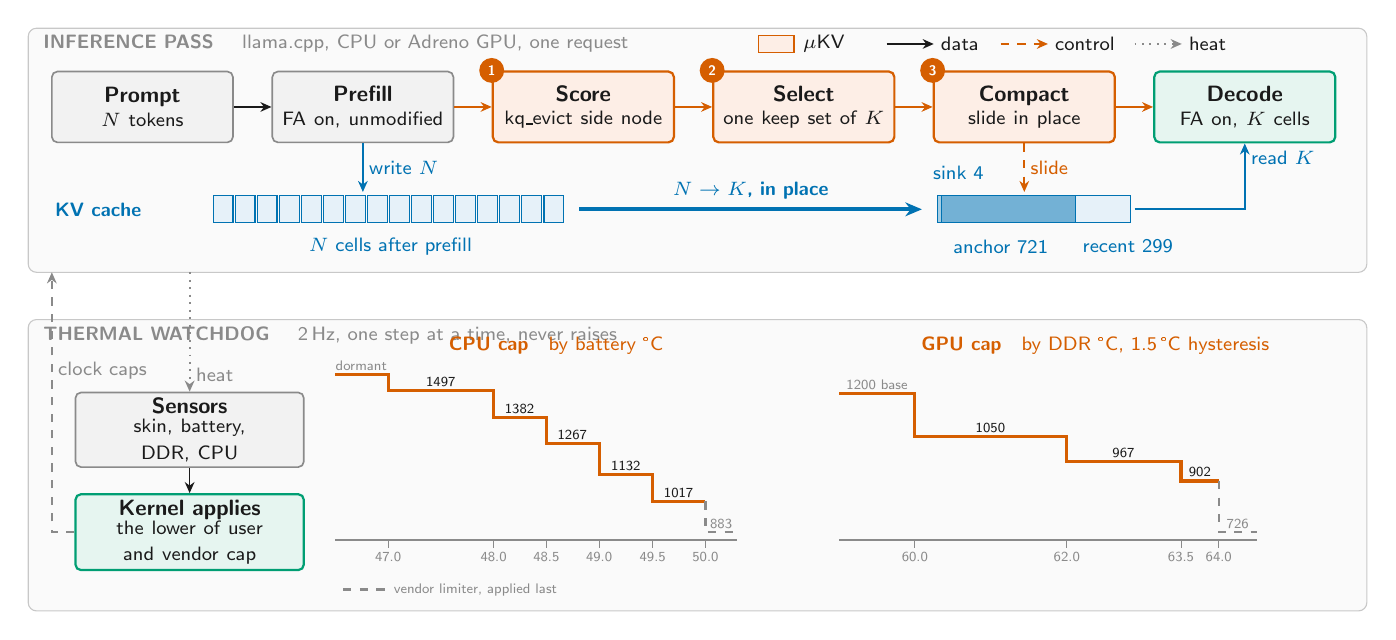
\begin{tikzpicture}[x=1cm,y=1cm]
% ================= panels =================
% ================= panels =================
\fill[panel,draw=pline,rounded corners=3pt] (0,4.35) rectangle (17,7.45);
\fill[panel,draw=pline,rounded corners=3pt] (0,0.05) rectangle (17,3.75);
\node[head,anchor=north west,text=gr] at (0.15,7.4) {INFERENCE PASS \quad {\mdseries llama.cpp, CPU or Adreno GPU, one request}};
\node[head,anchor=north west,text=gr] at (0.15,3.7) {THERMAL WATCHDOG \quad {\mdseries 2\,Hz, one step at a time, never raises}};
\draw[data] (10.9,7.25) -- (11.5,7.25);\node[lab,anchor=west] at (11.55,7.25) {data};
\draw[ctrl] (12.35,7.25) -- (12.95,7.25);\node[lab,anchor=west] at (13.0,7.25) {control};
\draw[heat] (14.05,7.25) -- (14.65,7.25);\node[lab,anchor=west] at (14.7,7.25) {heat};
\node[draw=or,fill=orf,minimum width=0.45cm,minimum height=0.22cm,inner sep=0] at (9.5,7.25) {};\node[lab,anchor=west] at (9.8,7.25) {$\mu$KV};
% ================= the pass =================
\node[box] (prompt) at (1.45,6.45) {\bx{Prompt}{$N$ tokens}};
\node[box] (prefill) at (4.25,6.45) {\bx{Prefill}{FA on, unmodified}};
\node[mukv] (score) at (7.05,6.45) {\bx{Score}{kq\_evict side node}};
\node[mukv] (select) at (9.85,6.45) {\bx{Select}{one keep set of $K$}};
\node[mukv] (compact) at (12.65,6.45) {\bx{Compact}{slide in place}};
\node[outc] (decode) at (15.45,6.45) {\bx{Decode}{FA on, $K$ cells}};
\draw[data] (prompt) -- (prefill);
\draw[data,or] (prefill) -- (score); \draw[data,or] (score) -- (select); \draw[data,or] (select) -- (compact); \draw[data,or] (compact) -- (decode);
\node[stepn] at (score.north west) {1};\node[stepn] at (select.north west) {2};\node[stepn] at (compact.north west) {3};
% KV strip
\node[lab,text=bl,font=\bfseries\scriptsize,anchor=west] at (0.3,5.15) {KV cache};
\foreach \i in {0,...,15}{\fill[blf,draw=bl,line width=0.4pt] (2.35+\i*0.28,4.98) rectangle (2.35+\i*0.28+0.25,5.32);}
\node[lab,text=bl] at (4.6,4.68) {$N$ cells after prefill};
\draw[kv] (prefill.south) -- (4.25,5.37) node[lab,text=bl,midway,right=1pt] {write $N$};
\draw[kv,line width=1.4pt,-{Stealth[length=6pt,width=5pt]}] (7.0,5.15) -- (11.35,5.15) node[lab,text=bl,font=\bfseries\scriptsize,midway,above=2pt] {$N \to K$, in place};
% compacted strip, proportional to the measured 4 / 721 / 299 split of K = 1024
\fill[bl!35!white,draw=bl,line width=0.4pt] (11.55,4.98) rectangle (11.60,5.32);
\fill[bl!55!white,draw=bl,line width=0.4pt] (11.60,4.98) rectangle (13.30,5.32);
\fill[blf,draw=bl,line width=0.4pt] (13.30,4.98) rectangle (14.00,5.32);
\node[lab,text=bl,anchor=west] at (11.45,5.62) {sink 4};
\node[lab,text=bl] at (12.35,4.68) {anchor 721};
\node[lab,text=bl,anchor=west] at (13.35,4.68) {recent 299};
\draw[ctrl] (compact.south) -- (12.65,5.37) node[lab,text=or,midway,right=1pt] {slide};
\draw[kv] (14.05,5.15) -- (15.45,5.15) -- (decode.south) node[lab,text=bl,pos=0.78,right=1pt] {read $K$};
% ================= control plane: the two ladders, drawn as ladders =================
\tikzset{colA/.style={box,minimum width=2.9cm,text width=2.7cm,minimum height=0.9cm},
         tread/.style={line width=1.1pt,or},
         vend/.style={line width=0.9pt,gr,dashed},
         axl/.style={font=\tiny,text=gr,inner sep=1pt},
         mhz/.style={font=\tiny,text=ink,inner sep=1pt}}
\node[colA] (sens) at (2.05,2.35) {\bx{Sensors}{skin, battery,\\ DDR, CPU}};
\node[colA,draw=gn,fill=gnf,line width=0.8pt] (appl) at (2.05,1.05) {\bx{Kernel applies}{the lower of user\\ and vendor cap}};
\draw[data] (sens) -- (appl);
\draw[vend] (4.00,0.32) -- (4.55,0.32); \node[lab,anchor=west,text=gr,font=\tiny] at (4.60,0.32) {vendor limiter, applied last};
% ---- CPU ladder: battery C -> prime-core cap
\node[head,text=or,anchor=west] at (5.30,3.42) {CPU cap \; {\mdseries by battery \textdegree C}};
\draw[gr,line width=0.4pt] (3.90,0.95) -- (9.00,0.95);
\draw[tread] (3.90,3.05) -- (4.57,3.05) -- (4.57,2.85) -- (5.91,2.85) -- (5.91,2.51) -- (6.58,2.51)
          -- (6.58,2.17) -- (7.25,2.17) -- (7.25,1.78) -- (7.93,1.78) -- (7.93,1.44) -- (8.60,1.44);
\draw[vend] (8.60,1.44) -- (8.60,1.05) -- (9.00,1.05);
\node[mhz,anchor=south,text=gr] at (4.23,3.06) {dormant};
\node[mhz,anchor=south] at (5.24,2.86) {1497};
\node[mhz,anchor=south] at (6.24,2.52) {1382};
\node[mhz,anchor=south] at (6.91,2.18) {1267};
\node[mhz,anchor=south] at (7.59,1.79) {1132};
\node[mhz,anchor=south] at (8.26,1.45) {1017};
\node[mhz,anchor=south,text=gr] at (8.80,1.06) {883};
\foreach \x/\t in {4.57/47.0, 5.91/48.0, 6.58/48.5, 7.25/49.0, 7.93/49.5, 8.60/50.0}
  {\draw[gr,line width=0.3pt] (\x,0.95) -- (\x,0.85); \node[axl,anchor=north] at (\x,0.83) {\t};}
% ---- GPU ladder: DDR C -> Adreno cap
\node[head,text=or,anchor=west] at (11.30,3.42) {GPU cap \; {\mdseries by DDR \textdegree C, 1.5\,\textdegree C hysteresis}};
\draw[gr,line width=0.4pt] (10.30,0.95) -- (15.60,0.95);
\draw[tread] (10.30,2.81) -- (11.26,2.81) -- (11.26,2.26) -- (13.19,2.26) -- (13.19,1.95) -- (14.64,1.95)
          -- (14.64,1.70) -- (15.12,1.70);
\draw[vend] (15.12,1.70) -- (15.12,1.05) -- (15.60,1.05);
\node[mhz,anchor=south,text=gr] at (10.78,2.82) {1200 base};
\node[mhz,anchor=south] at (12.22,2.27) {1050};
\node[mhz,anchor=south] at (13.91,1.96) {967};
\node[mhz,anchor=south] at (14.88,1.71) {902};
\node[mhz,anchor=south,text=gr] at (15.36,1.06) {726};
\foreach \x/\t in {11.26/60.0, 13.19/62.0, 14.64/63.5, 15.12/64.0}
  {\draw[gr,line width=0.3pt] (\x,0.95) -- (\x,0.85); \node[axl,anchor=north] at (\x,0.83) {\t};}
% ---- links between the panels
\draw[heat] (2.05,4.35) -- (sens.north) node[lab,text=gr,pos=0.86,right=1pt] {heat};
\draw[ctrlg] (appl.west) -- (0.30,1.05) -- (0.30,4.35) node[lab,text=gr,pos=0.62,right=1pt] {clock caps};
\end{tikzpicture}
\end{document}
